\documentclass[./main.tex]{subfiles}

\begin{document}
\section{Analisi discriminante}
\subsection*{LDA}
L\rq{}accuratezza raggiunta dall\rq{}analisi discriminante lineare nell\rq{}insieme di validazione è del $79.2\%$.
\begin{figure}[H]
	\centering
	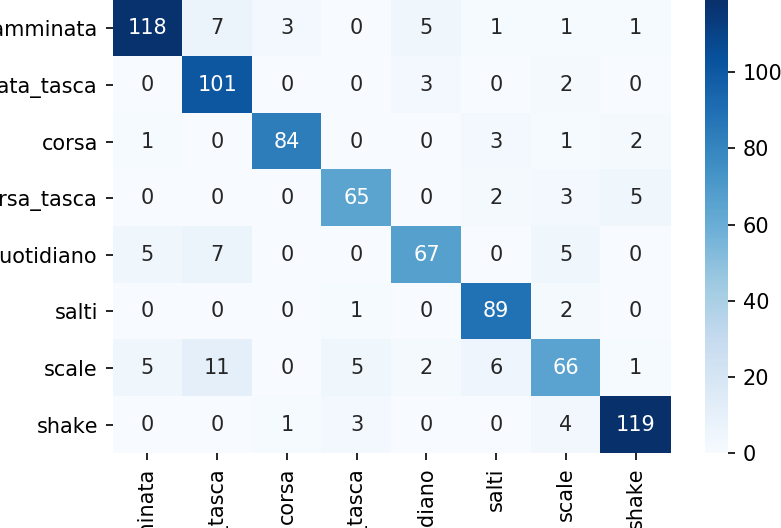
\includegraphics[width=.6\textwidth, keepaspectratio]{../../figure/confusionMatrix-QDA.png}
	\caption{{Matrice di confusione analisi discriminante lineare.}}
	\label{fig:lda}
\end{figure}

\subsection*{QDA}
L\rq{}accuratezza raggiunta dall\rq{}analisi discriminante quadratica nell\rq{}insieme di validazione è del $93.0\%$. Nonostante le esplicative non 
\begin{figure}[H]
	\centering
	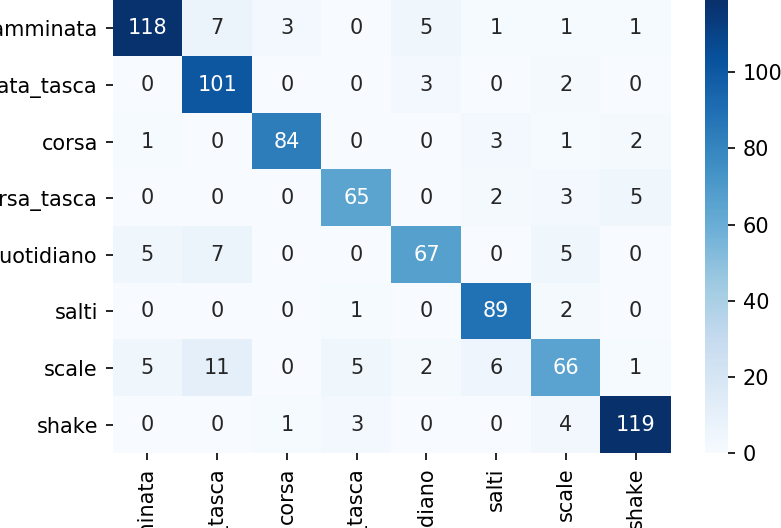
\includegraphics[width=.6\textwidth, keepaspectratio]{../../figure/confusionMatrix-QDA.png}
	\caption{{Matrice di confusione analisi discriminante quadratica.}}
	\label{fig:qda}
\end{figure}

\end{document}